\documentclass{article}
\usepackage[utf8]{inputenc}
\usepackage{graphicx}
\usepackage[margin=0.5in]{geometry}
\title{Stat490 Homework}
\author{ANDY LI}
\date{March 2023}

\begin{document}
\maketitle
Show $$E(MSA) = \sigma^2 + \frac{JK}{I-1} \sum_i \alpha_i^2$$
\\We know that $E(MSA) = E(\frac{SSA}{df_A}) = E(\frac{SSA}{I - 1})$
\\We also know that $$SSA = \sum_i JK(\hat{x}_i - \hat{x})^2 \Rightarrow JK\sum_i (\hat{x}_i^2 - 2\hat{x}_i\hat{x} + \hat{x}^2)$$
\\Hence by substituting, we get $$E(MSA) = E(\frac{JK}{I -1} \sum_i (\hat{x}_i^2 - 2\hat{x}_i\hat{x} + \hat{x}^2)) \Rightarrow \frac{JK}{I - 1} \sum_i (E[\hat{x}_i^2] - 2E[\hat{x}_i]E[\hat{x}] + E[\hat{x}^2]) \Rightarrow$$
$$\frac{JK}{I - 1} \sum_i (Var(\hat{x}_i) - E[\hat{x}_i]^2 - 2E[\hat{x}_i]E[\hat{x}] + var(\hat{x}) - E[\hat{x}]^2) \Rightarrow$$
$$E(MSA) = \sigma^2 + \frac{JK}{I - 1} \sum_i \alpha_i^2$$

\section*{5.6}
a) $DF_B = 3$
\\$SS_A = 0.0002$
\\$MS_B = SS_B / DF_B = 60.126$
\\$MS_{Interaction} = 8.479/3 = 2.8263$
\\$MSE = 19.8496$
\\F values are the corresponding MS divided by MSE.
\\$F_A = 0.0002 / 19.8496 = 0.00001$
\\$F_B = 3.0291$
\\$F_{Interaction} = 0.1424$
\\From the F table, we get the P values.
\\$P_A = 0.998$
\\$P_B = 0.093$
\\$P_{Interaction} = 0.932$
\\
\\b) 4 levels were used for factor B.
\\
\\c) 2 replicates of the experiment were performed.
\\
\\d) We can conclude that Factor B is significant at the $10\%$ significance level (p value of 0.093), but factor A and the interaction between A and B are not significant.

\section*{5.7}
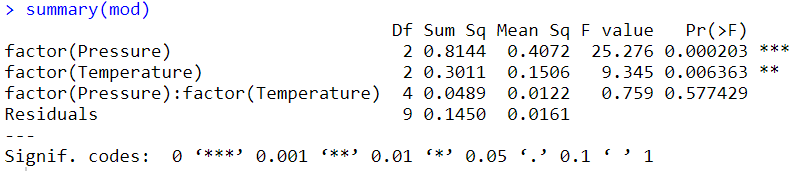
\includegraphics{5.7a.PNG}
\\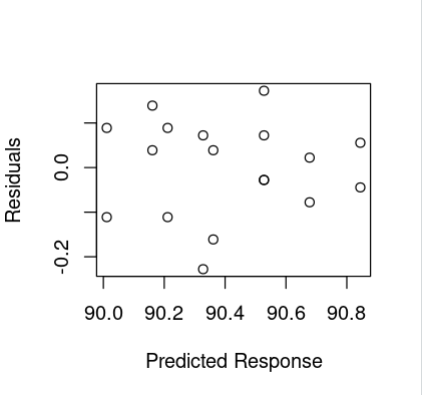
\includegraphics{5.7bRes.PNG} 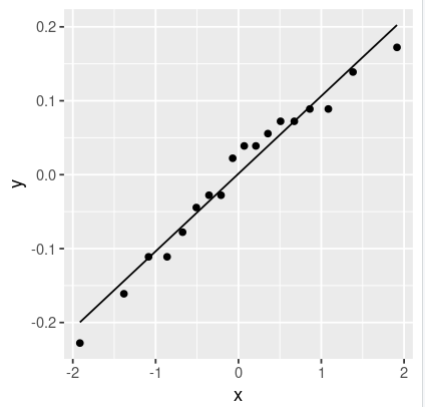
\includegraphics{5.7bQQ.PNG}
\\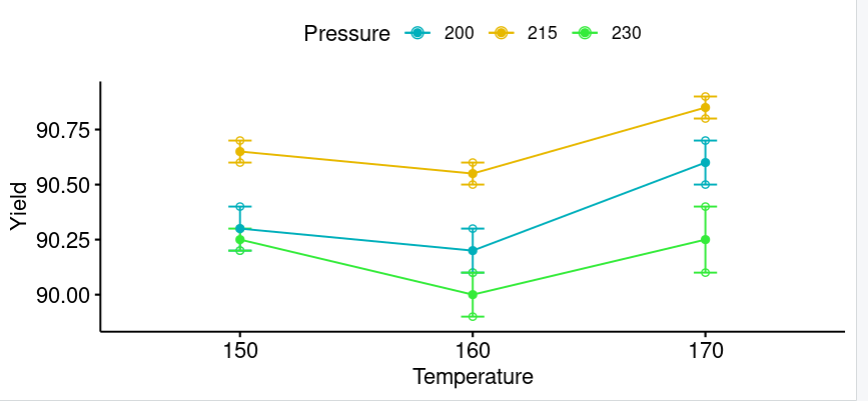
\includegraphics{5.7c.PNG}
\\To get the highest yield, we want to set pressure to 215, and temperature to 170.

\section*{5.13}
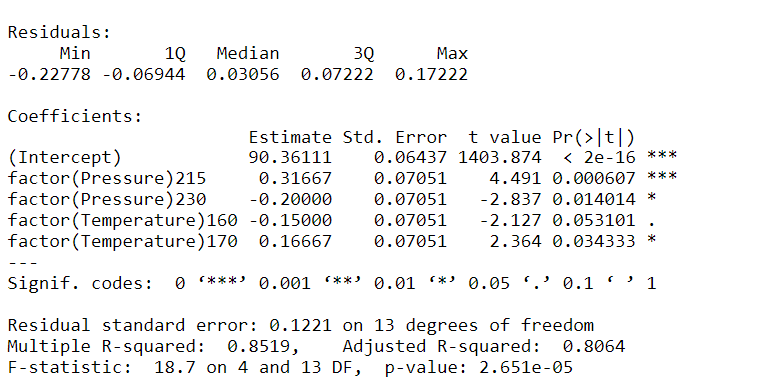
\includegraphics{5.13.PNG}
\\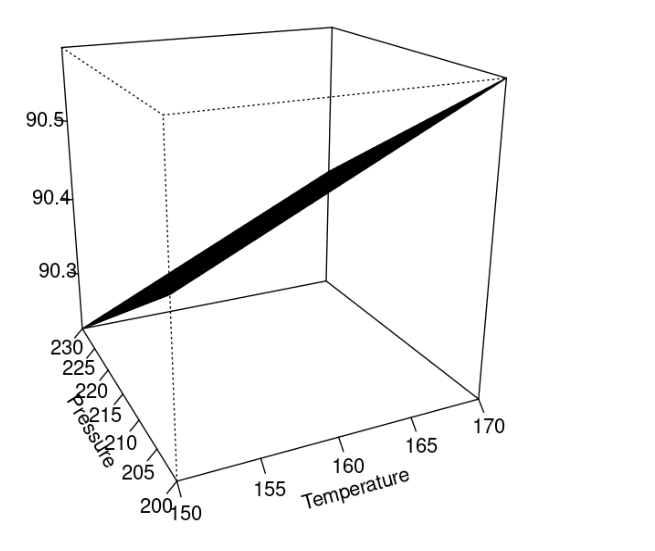
\includegraphics{5.13persp.PNG}
\\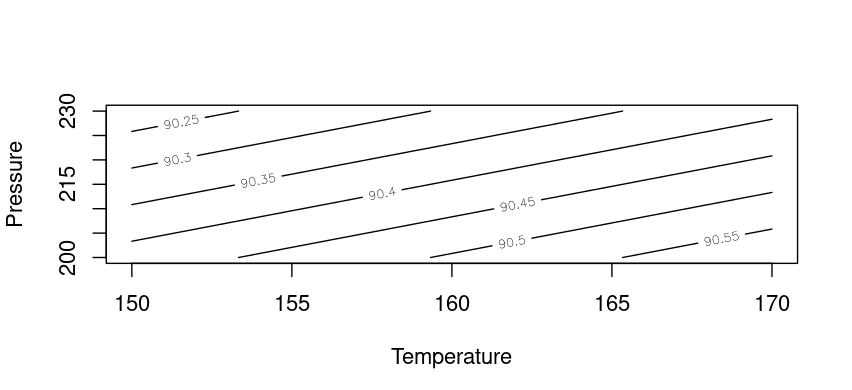
\includegraphics{5.13cont.PNG}

\section*{5.14}
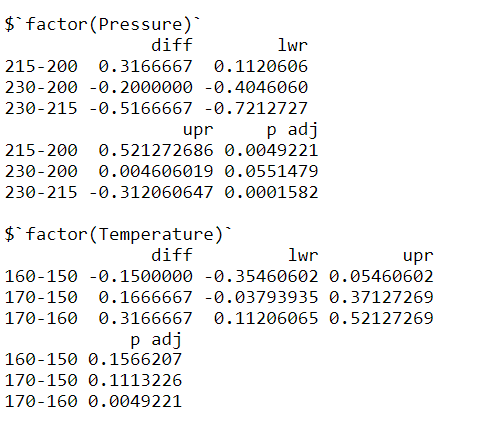
\includegraphics{5.14.PNG}
\\For the Pressure factor, we primarily see a difference of means between 215 and both 200 and 230 pressures.

\section*{5.18}
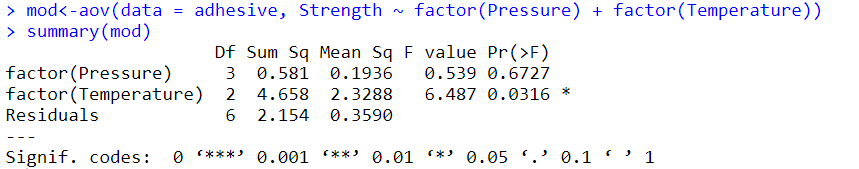
\includegraphics{5.18a.PNG}
\\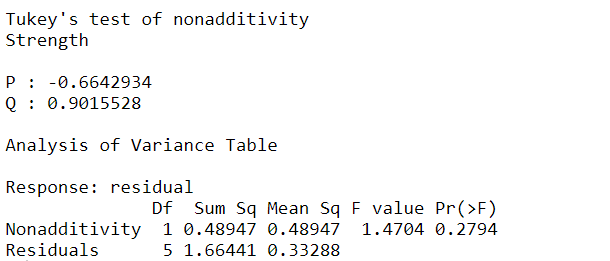
\includegraphics{5.18b.PNG}
\\Temperature is the significant factor at the 0.05 significance level.
\\The test for nonadditivity returns a p value of 0.2794 which is greater than 0.05.

\section*{5.26}
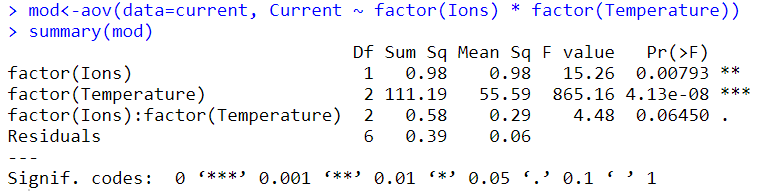
\includegraphics{5.26a.PNG}
\\At the 0.05 significance level, both doping and temperature are significant. However, their interaction is not significant at the 0.05 significance level.
\\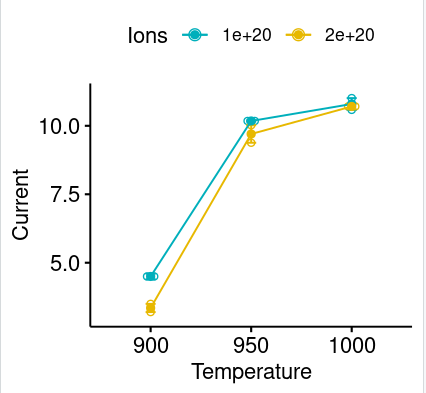
\includegraphics{5.26b.PNG}
\\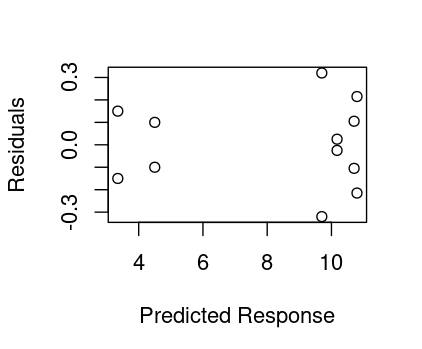
\includegraphics{5.26cRes.PNG}
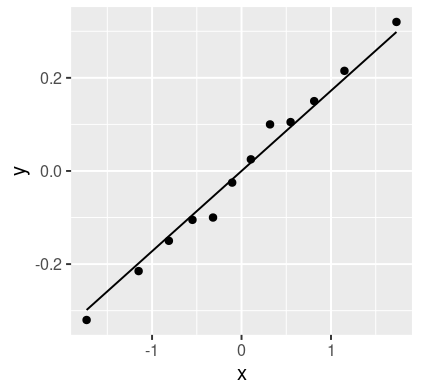
\includegraphics{5.26cQQ.PNG}
\\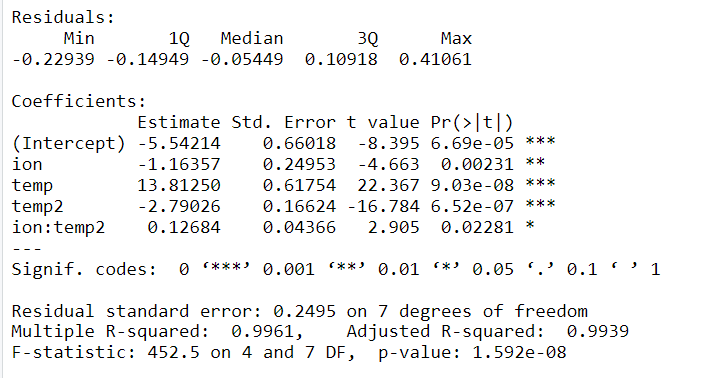
\includegraphics{5.26dlm.PNG}

\section*{5.29}
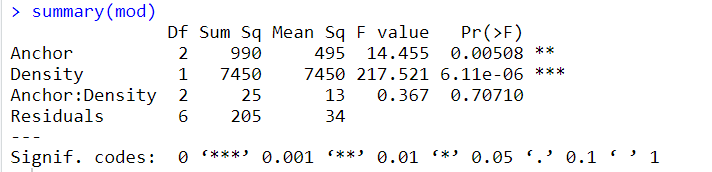
\includegraphics{5.29a.PNG}

\\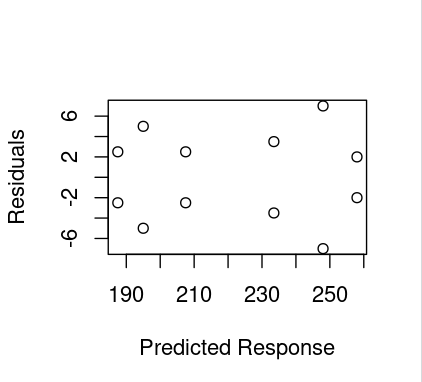
\includegraphics{5.29bRes.PNG} 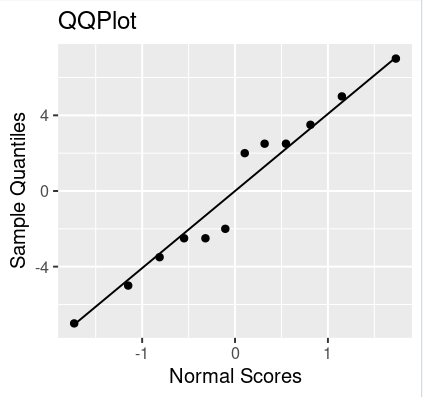
\includegraphics{5.29bQQ.PNG}
\\We can conclude that both Anchor and Density are significant at the 0.05 confidence level. However their interaction is not significant at the 0.05 confidence level.

\section*{5.39}
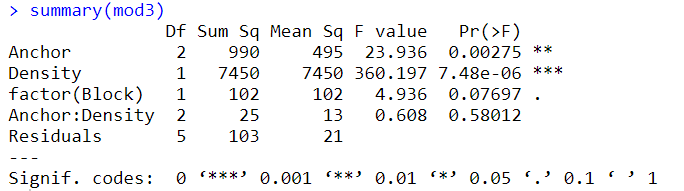
\includegraphics{5.39.PNG}
\\Compared to the factorial design, the factorial blocking design does not seem too useful.
$$\hat{\sigma}_\beta^2 = \frac{MS_B - MS_E}{ab} = \frac{103 - 21}{6} = 13.67$$

\section*{6.9}
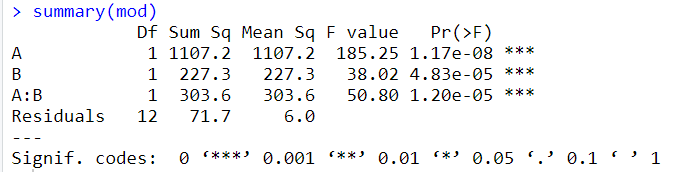
\includegraphics{6.9a.PNG}
\\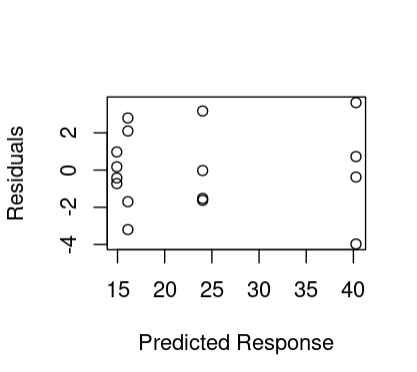
\includegraphics{6.9bRes.PNG} 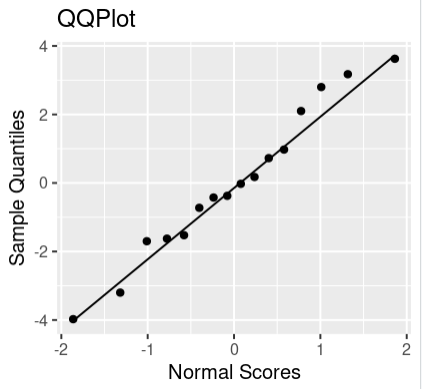
\includegraphics{6.9bQQ.PNG}
\\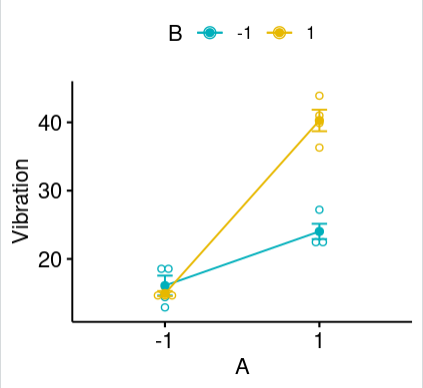
\includegraphics{6.9c.PNG}
\\Note: A: Bit Size, B: Cutting Speed.
\\In order to reduce vibration, a smaller bit size is preferred. When using a small bit size, both cutting speeds produce similar vibrations. Hence, in order to reduce vibrations, the recommended bit size is small.

\section*{6.14}
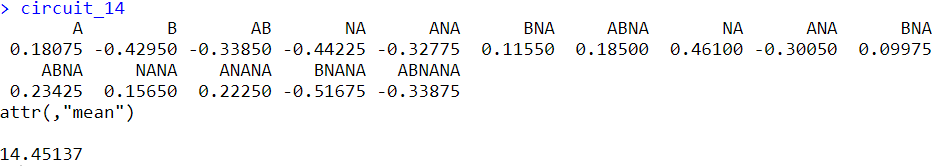
\includegraphics{6.14a.PNG}
\\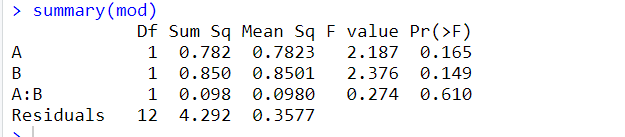
\includegraphics{6.14b.PNG}
\\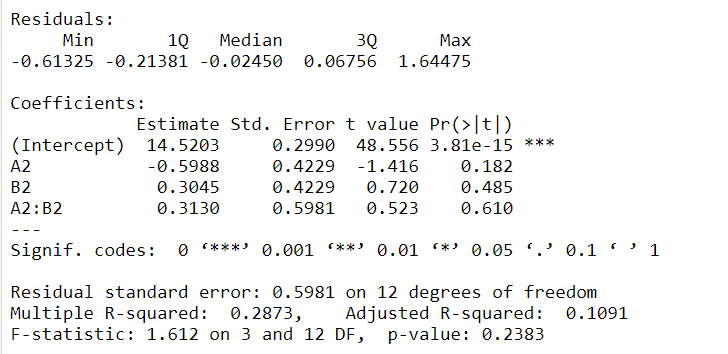
\includegraphics{6.14c.PNG}

\section*{6.15}
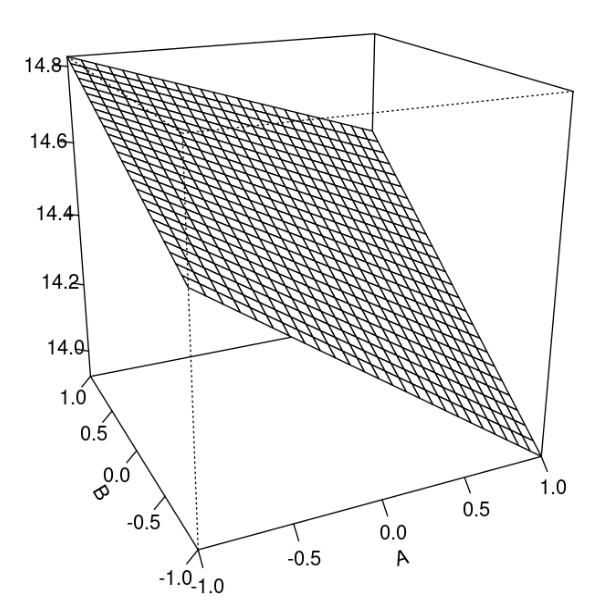
\includegraphics{6.15persp.PNG}
\\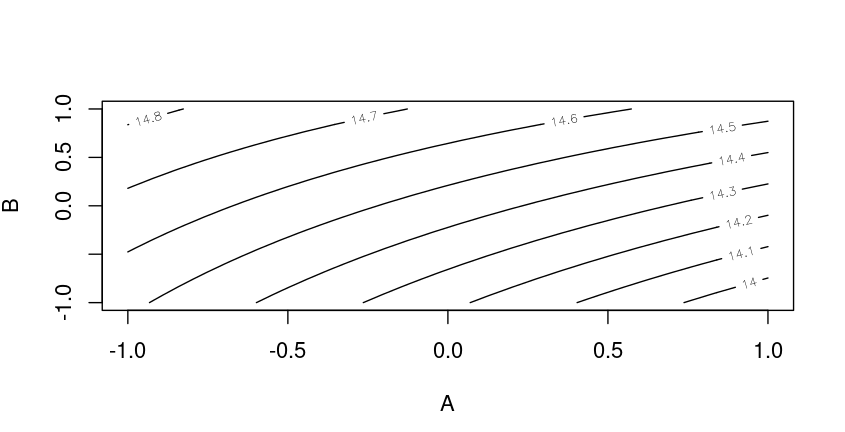
\includegraphics{6.15cont.PNG}
\newpage
\section*{6.33}
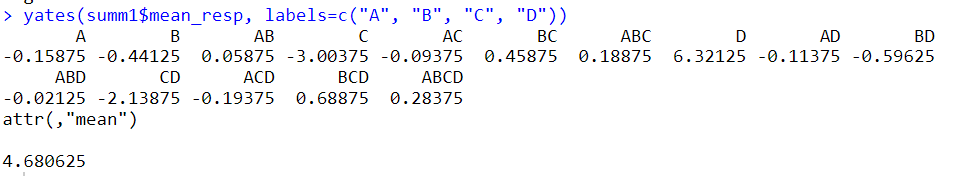
\includegraphics{6.33a.PNG}
\\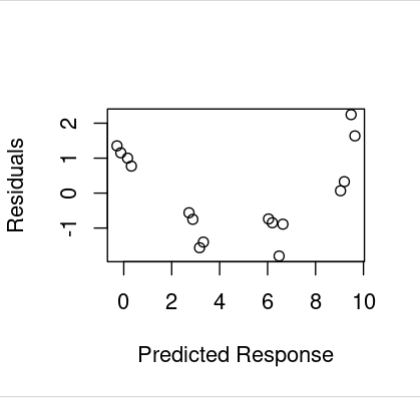
\includegraphics{6.33bRes.PNG} 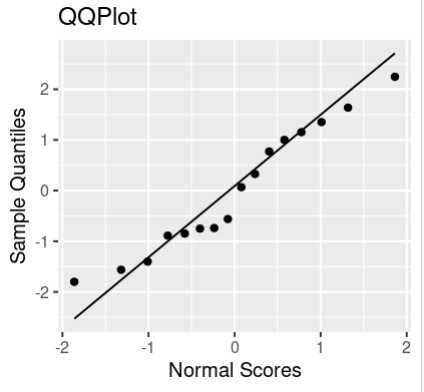
\includegraphics{6.33bQQ.PNG}
\\Yes, according to the residual plots the data does not seem to be normal.
\\
\\After taking $ln(Resistivity)$
\\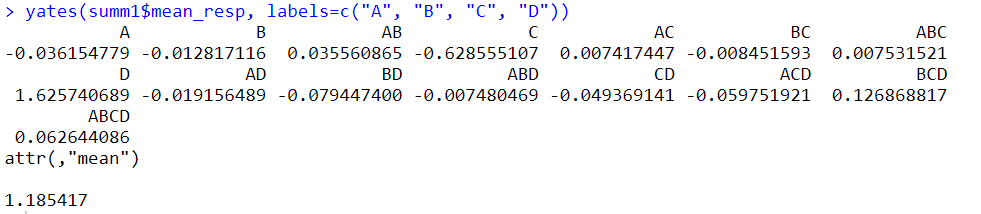
\includegraphics{6.33c1.PNG}
\\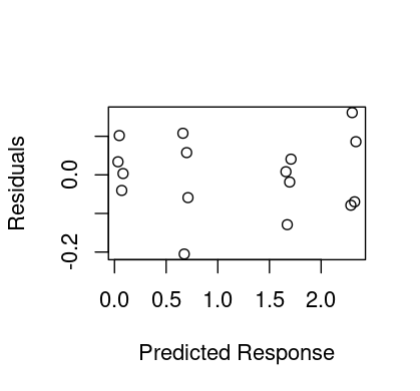
\includegraphics{6.33cRes.PNG} 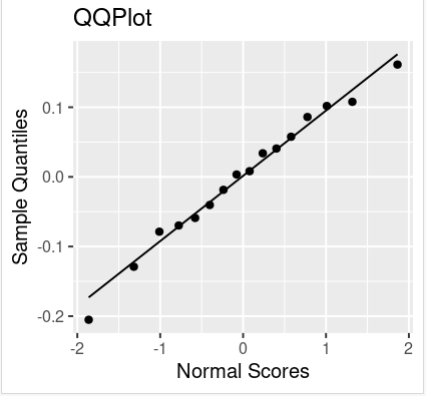
\includegraphics{6.33cQQ.PNG}
\\The transformation is useful because it makes the distribution approximately normal as shown by the transformed residual and QQ plots.
\\
\\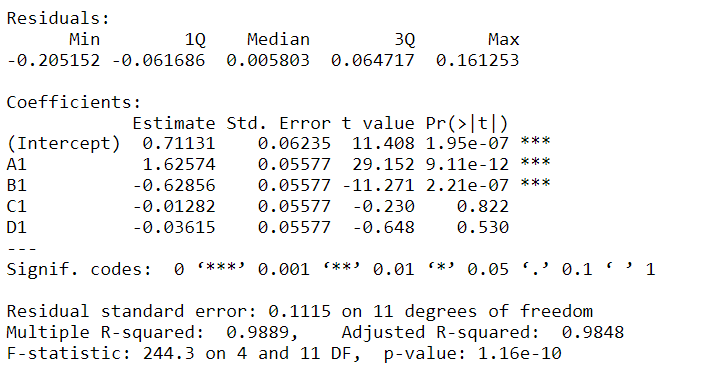
\includegraphics{6.33d.PNG}
\end{document}